\documentclass{article}

\usepackage[preprint]{neurips_2025}

\usepackage[utf8]{inputenc}
\usepackage[T1]{fontenc}
\usepackage{hyperref}
\usepackage{url}
\usepackage{booktabs}
\usepackage{tabularx}
\usepackage{amsmath}
\usepackage{amsfonts}
\usepackage{microtype}
\usepackage{xcolor}
\usepackage{graphicx}
\usepackage{caption}
\usepackage{subcaption}
\usepackage{multirow}
\usepackage{float}

\hypersetup{colorlinks=true, linkcolor=black, citecolor=blue!60!black, urlcolor=blue!60!black}
\setcitestyle{numbers,square,comma}
\newcolumntype{Y}{>{\raggedright\arraybackslash}X}
\captionsetup{font=small}
\renewcommand{\topfraction}{0.85}
\renewcommand{\textfraction}{0.1}
\renewcommand{\floatpagefraction}{0.75}

% Match the course reference layout: no title rules, no conference footer.
\makeatletter
\setlength{\parskip}{4\p@}
\renewcommand{\@toptitlebar}{\vskip 0.05in}
\renewcommand{\@bottomtitlebar}{\vskip 0.05in}
\renewcommand{\@noticestring}{}
\makeatother

\newcommand{\pp}{\,pp}
\newcommand{\ci}[2]{[$#1$, $#2$]}
\newcommand{\takeaway}[1]{\paragraph{#1}}

\title{Fade, Don't Forget:\\Low-Bit Attention Memory for Hybrid Reasoning Models}

\author{%
  Vu Hai An \\
  GStar Bootcamp 2026 \\
  \texttt{vuhaiandp2017@gmail.com} \\
  Code: \url{https://github.com/haian1910/Gstar_2026_Individual_Project}
}

\begin{document}

\maketitle

\vspace{-1.5em}
\begin{abstract}
Reasoning models write tens of thousands of tokens per answer, and the attention cache that stores this text dominates their memory. Hybrid models such as Qwen3.5 replace most attention layers with recurrent layers of fixed size, but the few attention layers that remain still store every token, and in Qwen3.5-9B they hold 95\% of a sample's memory (analytic) at 32K tokens. Simply forgetting old tokens does not work: in our earlier project it cost 40 points of math accuracy. We propose \emph{Fade}: keep the prompt and the most recent tokens exact, and store all older tokens at 2 or 4 bits. Fade needs no training and leaves the recurrent layers untouched. On 120 competition math problems, 4-bit Fade shows no detectable loss against full attention with just over a third of its analytic memory. 2-bit Fade loses about 6 points, but it beats an 8K window that keeps the prompt, with 30\% less analytic memory (a modest gain; a post hoc split puts all of it in one of two seed pairs), and it is far better than StreamingLLM (2 samples per problem). When 2-bit Fade fails, the model does not give wrong answers; it reasons for longer and runs out of tokens. Accuracy comes from emulated quantization; memory is analytic, and a benchmark with real packed storage agrees with it to within the pre-registered 10\%; we make no speed claim. Code and run data: \url{https://github.com/haian1910/Gstar_2026_Individual_Project}.
\end{abstract}

\vspace{-0.6em}
\section{Introduction}
\vspace{-0.4em}
Long chains of thought buy accuracy with tokens: competition math traces run to 20K--30K tokens. During generation, the model stores the keys and values (KV) of every token so that later tokens can attend to them, and this \emph{KV cache} grows with every token. \emph{Hybrid} models reduce this cost by replacing most attention layers with linear recurrent layers, which summarize the past in a fixed-size state. Qwen3.5-9B~\cite{qwen35} repeats a block of 3 Gated DeltaNet (GDN)~\cite{gdn} layers and 1 full-attention (FA) layer 8 times (Figure~\ref{fig:hybrid}a). The 24 GDN layers keep a fixed 49\,MiB state per sample, but the 8 FA layers still cache 32\,KiB per token: at 32K tokens that is 1\,GiB, 95\% of the sample's analytic memory (Figure~\ref{fig:hybrid}b).

\begin{figure}[h]
\centering
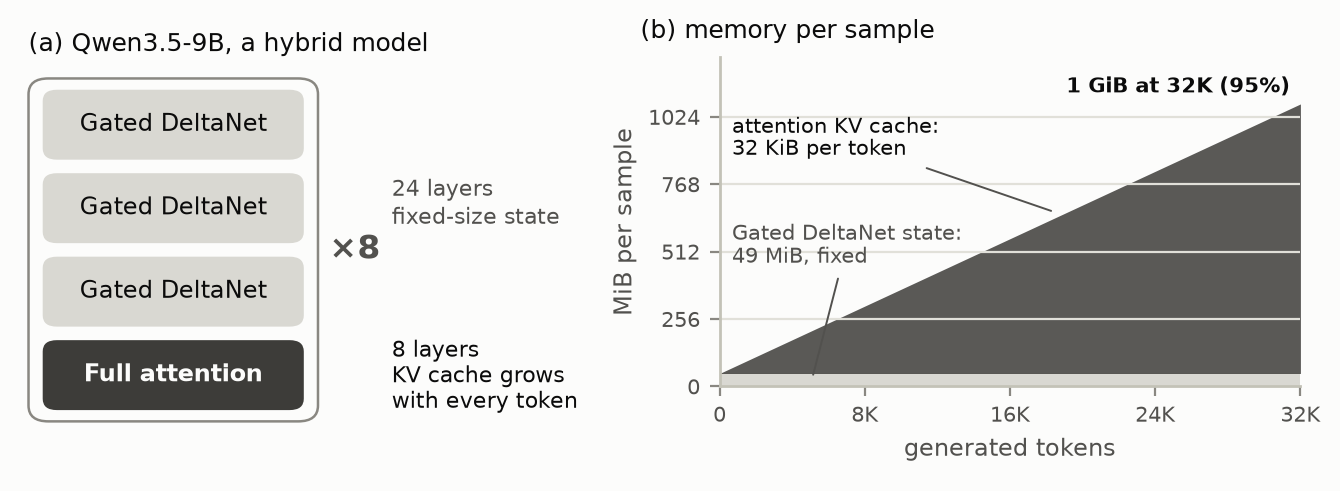
\includegraphics[width=0.92\linewidth]{figures/fig_fade_hybrid.png}
\vspace{-0.5em}
\caption{The problem. (a) Qwen3.5-9B is a hybrid: most layers are Gated DeltaNet layers with a fixed-size state; one layer in four is full attention. (b) Memory per sample as the model writes (analytic): the attention KV cache grows with every token and dominates; the GDN state stays at 49\,MiB.}
\label{fig:hybrid}
\vspace{-0.6em}
\end{figure}

The obvious fix is to forget. In our previous project, Think-Local, the FA layers saw only the prompt and the last 2K generated tokens. Math accuracy fell by 40 points. The runs that finished were almost always right; the loss came from runs that never finished within the token limit. Exploratory attention maps (not audited) suggest that no small fix exists: every attention head reads far back into the trace, so there is no small set of ``long-range'' heads to keep exact (Appendix~\ref{app:tl}).

If every head needs old tokens, a cheaper memory has to keep all of them, just less precisely. \emph{Fade} keeps the prompt and the recent tokens exact and stores everything older at 2 or 4 bits (Figure~\ref{fig:schematic}). We ask two questions: how close does Fade come to full attention, and how does it compare, at matched memory, with the standard ways to bound the cache? Our contributions:
\begin{itemize}\setlength{\itemsep}{1pt}\setlength{\topsep}{0pt}
\item \textbf{Fade}, a training-free memory policy for the attention layers of a hybrid model. At 32K tokens its analytic memory per sample falls from 1,073\,MiB to 368\,MiB (4-bit) or 248\,MiB (2-bit), and a benchmark with real packed low-bit storage matches this accounting to within 10\%.
\item \textbf{A pre-registered comparison} on Qwen3.5-9B: 4-bit Fade shows no detectable loss against full attention; 2-bit Fade beats an 8K window that keeps the prompt at 0.70$\times$ its analytic memory (a post hoc split puts the whole gain on one of two seed pairs), and it is far better than StreamingLLM~\cite{streamingllm}.
\item \textbf{How a low-bit memory fails}: the model still answers correctly when it finishes, but it reasons for longer and hits the token limit more often, mainly on the longest problems (exploratory).
\end{itemize}

\vspace{-0.6em}
\section{Related Work}
\vspace{-0.4em}
\paragraph{KV-cache quantization.} KIVI~\cite{kivi} quantizes keys per channel and values per token and keeps the most recent tokens in full precision; Fade uses this quantizer. KVQuant~\cite{kvquant} quantizes keys before RoPE, SKVQ~\cite{skvq} keeps a sliding window of exact recent tokens, and rotations spread outliers before quantizing (QuaRot~\cite{quarot}, QJL~\cite{qjl}, TurboQuant~\cite{turboquant}). We do not propose a new quantizer; any of these could replace KIVI inside Fade (untested). What is new is where it is applied (only the attention layers of a hybrid, with the prompt exact) and the test: long reasoning, against eviction at matched memory.

\paragraph{KV compression for long reasoning.} R-KV~\cite{rkv} and RaaS~\cite{raas} evict redundant or finished tokens during decoding. PM-KVQ~\cite{pmkvq} lowers bit-widths progressively; ThinKV~\cite{thinkv} mixes quantization and eviction by thought type and reports that aggressive compression lengthens reasoning. Closest to us, BreadthKV~\cite{breadthkv} finds on dense reasoning models that, at a matched byte budget, keeping more tokens at lower precision beats eviction, mainly by reducing runs that hit the length limit. We test the same trade-off in a hybrid, where only one layer in four has a growing cache. Our eviction baselines choose tokens by position; we do not compare with score-based eviction such as R-KV.

\paragraph{Windows, heads and hybrids.} StreamingLLM~\cite{streamingllm} keeps a few attention-sink tokens and a recent window. In dense models only some heads need long context, which retrieval heads~\cite{retrievalheads}, DuoAttention~\cite{duoattention} and RazorAttention~\cite{razorattention} exploit; our maps of Qwen3.5's FA heads find no such split. Delethink~\cite{delethink} and ThinkReset~\cite{thinkreset} train the model to reason in bounded chunks; Fade needs no training. Hybrids with about one attention layer in four include Qwen3.5~\cite{qwen35} and Kimi Linear~\cite{kimilinear}.

\vspace{-0.6em}
\section{Method}
\vspace{-0.4em}
\begin{figure}[t]
\centering
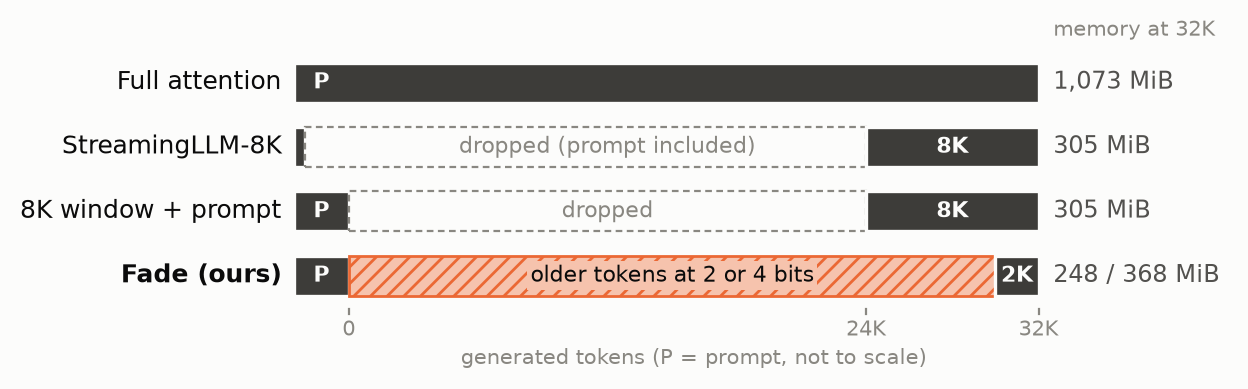
\includegraphics[width=0.92\linewidth]{figures/fig_fade_schematic.png}
\vspace{-0.6em}
\caption{What the attention layers keep of one 32K-token reasoning trace. Dark: exact (bf16); hatched: 2 or 4 bits; dashed: dropped. The GDN layers see every token in all four cases. Memory per sample at 32K is analytic (FA cache + 49\,MiB GDN state), with the prompt's KV left out because samples share it.}
\label{fig:schematic}
\vspace{-0.8em}
\end{figure}

\paragraph{Fade.} In every FA layer, prompt tokens stay exact. Generated tokens are grouped into blocks of 128. Once a block is more than $R{=}2{,}048$ tokens old, it is quantized to $b$ bits, once and for good, so the most recent ${\sim}$2K generated tokens are always exact. The GDN layers run unchanged over all tokens. There is no training and no calibration.

\paragraph{Quantizer.} We use the KIVI-style~\cite{kivi} asymmetric uniform quantizer: keys are quantized per channel and values per token, in groups of 128, each group with its own scale and zero point (adding 0.25 bits per element). A variant first rotates each head vector with a Hadamard matrix to spread outliers. Before attention the codes are dequantized, and attention runs in bf16 as usual.

\paragraph{Memory.} Each token costs 32\,KiB across the 8 FA layers when exact (4 KV heads of dimension 256 per layer). After $n$ generated tokens, a sample holds
\begin{equation}
M(n) = 32\,\text{KiB}\times\Big(n_{\text{exact}} + n_{\text{old}}\,\tfrac{b+0.25}{16}\Big) + 49.1\,\text{MiB},
\label{eq:mem}
\end{equation}
where $n_{\text{old}}$ counts the quantized tokens. At 32K tokens: full attention 1,073\,MiB, 8K window 305\,MiB, 4-bit Fade 368\,MiB, 2-bit Fade 248\,MiB.

\paragraph{Emulation.} For the accuracy runs we quantize and immediately dequantize blocks in place in the bf16 cache. The model therefore sees exactly what real $b$-bit storage would give it, but these runs save no memory. A separate benchmark stores real packed codes to check Eq.~\ref{eq:mem} (Section~\ref{sec:results}). Correctness checks are in Appendix~\ref{app:impl}.

\paragraph{Choosing two configurations.} Before any decoding, a fixed rule picked the configurations from a cheap teacher-forced sweep on 40 held-out traces, scoring how far each policy moves the next-token distribution (KL divergence; Appendix~\ref{app:kl}). It picked \textbf{Fade-2} (2-bit, Hadamard variant) and, since no 1-bit variant came close, the pre-registered fallback \textbf{Fade-4} (4-bit, plain).

\begin{figure}[t]
\centering
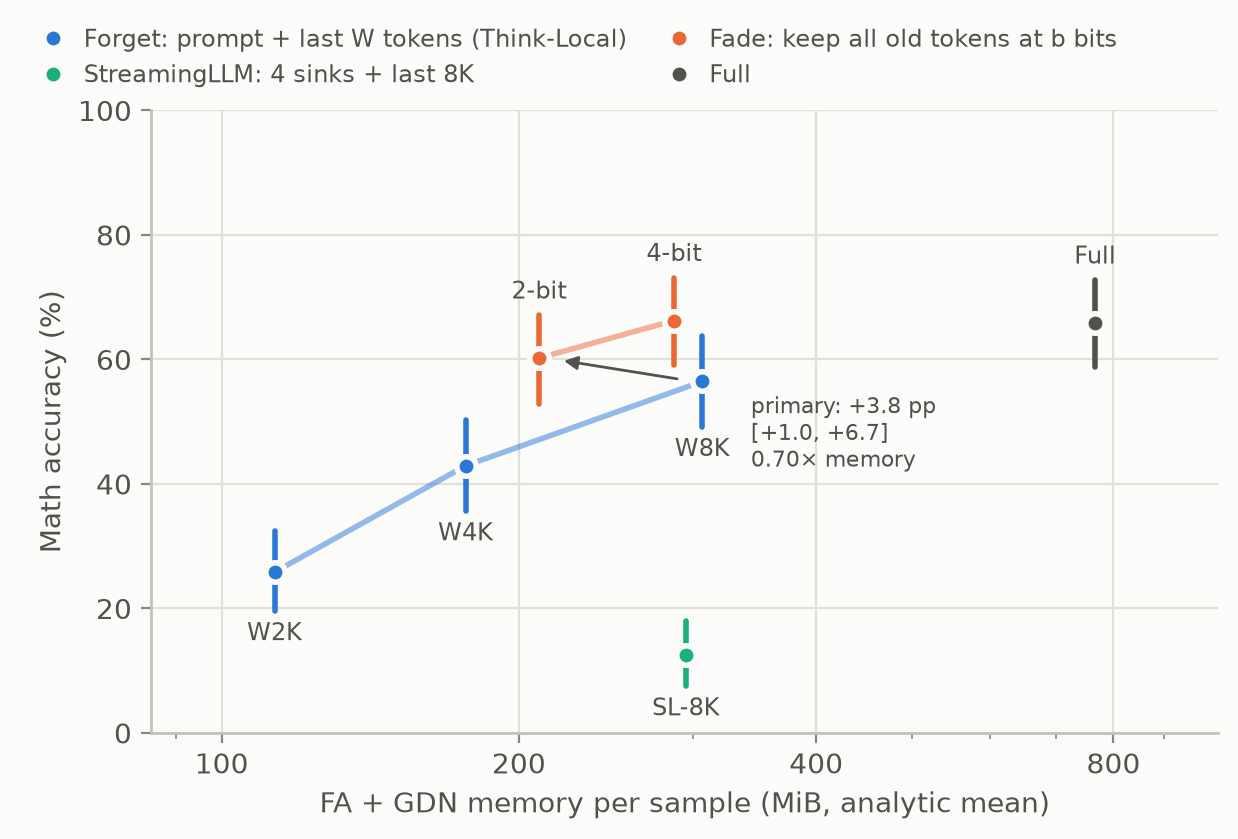
\includegraphics[width=0.66\linewidth]{figures/fig_fade_frontier.png}
\vspace{-0.6em}
\caption{Accuracy vs memory. Forgetting (blue: prompt + last $W$ tokens) loses accuracy fast as memory shrinks; Fade (orange) stays close to full attention. StreamingLLM-8K (green) drops the prompt too and collapses. Bars are 95\% CIs; the arrow is the pre-registered primary comparison. 4 samples per cell; StreamingLLM-8K 2. Memory is the analytic mean per sample over each run; the 8K window is drawn 3\% to the right so it does not hide Fade-4.}
\label{fig:frontier}
\vspace{-0.6em}
\end{figure}

\vspace{-0.6em}
\section{Experiments}
\vspace{-0.4em}
\subsection{Setup}
\vspace{-0.3em}
\textbf{Data.} 120 competition math problems, 30 from each of AIME 2025, AIME 2026 and HMMT February 2025 (via MathArena~\cite{matharena}) and MATH-500 level 5~\cite{hendrycksmath,math500}, the same set as Think-Local. \textbf{Decoding.} Qwen3.5-9B in thinking mode, sampling at temperature 1.0, with a 32,768-token limit and 4 samples per problem. A run that hits the limit counts as wrong. \textbf{Statistics.} Every comparison is paired by problem, with 95\% confidence intervals (CIs) from a bootstrap over problems. \textbf{Pre-registration.} The questions, the primary comparison (Fade-2 vs the 8K window at matched memory) and the wording of each verdict were fixed before any decode result, and an independent audit agent reproduced every decode number from the raw runs. Analyses added later are labelled post hoc or exploratory. Full details are in Appendix~\ref{app:impl}.

\subsection{Baselines}
\vspace{-0.3em}
All baselines use the same model, decoding loop and scorer, and change only what the FA layers attend to; the GDN layers always see all tokens.
\begin{itemize}\setlength{\itemsep}{1pt}\setlength{\topsep}{0pt}
\item \textbf{Full attention:} the exact cache (the upper bound).
\item \textbf{Windows that keep the prompt (2K, 4K, 8K):} the prompt plus the last $W$ generated tokens, from Think-Local. The \textbf{8K window} is the pre-registered matched-memory comparator.
\item \textbf{StreamingLLM-8K}~\cite{streamingllm}: 4 ``sink'' tokens plus the last 8,192 tokens, so the prompt is dropped once the window fills. Added after the project was refocused; its analysis was registered before any of its runs. Run with 2 samples per problem; its comparisons use the same 2 samples of every cell.
\end{itemize}

\subsection{Implementation Details}
\vspace{-0.3em}
The decoding loop uses Hugging Face Transformers with the \texttt{fla} kernels for GDN, in bf16, with continuous batching, on NVIDIA A100-80GB GPUs. Each cell has 480 runs (120 problems $\times$ 4 samples; 240 for StreamingLLM-8K). The full-attention and window runs are reused from Think-Local; Fade's runs used a later build of the same loop. This project's runs took about 16 GPU-hours plus 2.7 for StreamingLLM-8K and 0.5 for the memory benchmark, on the lab's own GPUs (Appendix~\ref{app:prereg}).

\vspace{-0.6em}
\section{Results}
\label{sec:results}
\vspace{-0.4em}

\begin{table}[t]
\caption{Main results on 120 math problems (32K-token limit, 4 samples per problem; StreamingLLM-8K: 2). Memory is analytic per sample (Eq.~\ref{eq:mem}): the mean over each run and the value at 32K tokens.}
\label{tab:main}
\centering
\small
\setlength{\tabcolsep}{4pt}
\begin{tabular}{@{}llrrcr@{}}
\toprule
Method & Older tokens & \multicolumn{2}{c}{MiB / sample} & Accuracy \% [95\% CI] & Hit limit \\
 & & mean & at 32K & & \% \\
\midrule
Full attention & exact & 766 & 1,073 & 65.8 [58.8, 72.7] & 34.0 \\
\textbf{Fade-4 (ours)} & \textbf{4 bits} & 287 & 368 & \textbf{66.2} [59.2, 73.1] & 33.1 \\
\textbf{Fade-2 (ours)} & \textbf{2 bits} & 210 & 248 & \textbf{60.2} [52.9, 67.1] & 39.8 \\
8K window + prompt & dropped & 298 & 305 & 56.5 [49.2, 63.7] & 43.3 \\
4K window + prompt & dropped & 177 & 177 & 42.9 [35.6, 50.2] & 57.1 \\
2K window + prompt & dropped & 113 & 113 & 25.8 [19.6, 32.5] & 74.2 \\
StreamingLLM-8K & dropped, prompt too & 295 & 305 & 12.5 [7.5, 17.9] & 43.3 \\
\bottomrule
\end{tabular}
\vspace{-0.4em}
\end{table}

\begin{table}[t]
\caption{Key paired comparisons (accuracy difference in percentage points, 95\% CI). Memory: ratio of analytic mean memory per sample. StreamingLLM rows use the same 2 samples per problem for both methods; their memory ratio leaves out the prompt's KV, which Fade keeps, so counting it the ratio is slightly higher. All comparisons are in Appendix~\ref{app:details}.}
\label{tab:contrasts}
\centering
\small
\setlength{\tabcolsep}{4pt}
\begin{tabularx}{\linewidth}{@{}llcY@{}}
\toprule
Comparison & Difference [95\% CI] & Memory & Verdict \\
\midrule
Fade-4 $-$ Full & $+0.4$ \ci{-2.7}{+3.5} & 0.37$\times$ & no detectable difference \\
Fade-2 $-$ Full & $-5.6$ \ci{-8.8}{-2.7} & 0.27$\times$ & worse; not shown non-inferior (5\pp\ margin) \\
\textbf{Fade-2 $-$ 8K window (primary)} & $+3.8$ \ci{+1.0}{+6.7} & 0.70$\times$ & better at matched memory; all of the gain in one of two seed pairs (post hoc) \\
Fade-2 $-$ StreamingLLM-8K & $+49.2$ \ci{+41.2}{+57.1} & 0.71$\times$ & better at matched memory \\
\bottomrule
\end{tabularx}
\vspace{-0.8em}
\end{table}

Figure~\ref{fig:frontier} shows the main picture, Table~\ref{tab:main} the numbers and Table~\ref{tab:contrasts} the key comparisons. We go through the findings one at a time.

\takeaway{1. 4-bit Fade: no detectable loss at 37\% of the analytic memory.} 4-bit Fade scores 66.2\% against full attention's 65.8\% ($+0.4$\pp, CI $-2.7$ to $+3.5$), with no detectable change in the rate of runs hitting the limit (33.1\% vs 34.0\%). The CI excludes a loss larger than 2.7 points; it does not prove the two are equal.

\takeaway{2. 2-bit Fade costs a few points but beats forgetting at matched memory.} Against full attention, 2-bit Fade loses 5.6 points at 27\% of the analytic memory, so it is not a free lunch. Against the 8K window, the pre-registered comparison, it is better by 3.8 points (CI $+1.0$ to $+6.7$) with 0.70$\times$ the analytic memory. The gain is modest: a post hoc split by seed pair puts all of it in seeds 0--1 ($+7.9$\pp), with no detectable difference in seeds 2--3 ($-0.4$\pp). Going from 0 to 2 bits per old token recovers 34 of the 40 points that the 2K window loses (Q2 curve; descriptive).

\takeaway{3. Dropping the prompt is much worse.} StreamingLLM-8K keeps the same number of recent tokens as the 8K window but drops the prompt, and it reaches only 12.5\%. 2-bit Fade beats it by 49.2 points with 0.71$\times$ its analytic memory (slightly more if the prompt's KV, which Fade keeps, is counted). Unlike every other method, most of its finished runs are wrong (Figure~\ref{fig:outcomes}a), and almost all of these (104 of 106) give no parsable answer once the prompt has been dropped; we do not test why (Appendix~\ref{app:details}).

\begin{figure}[t]
\centering
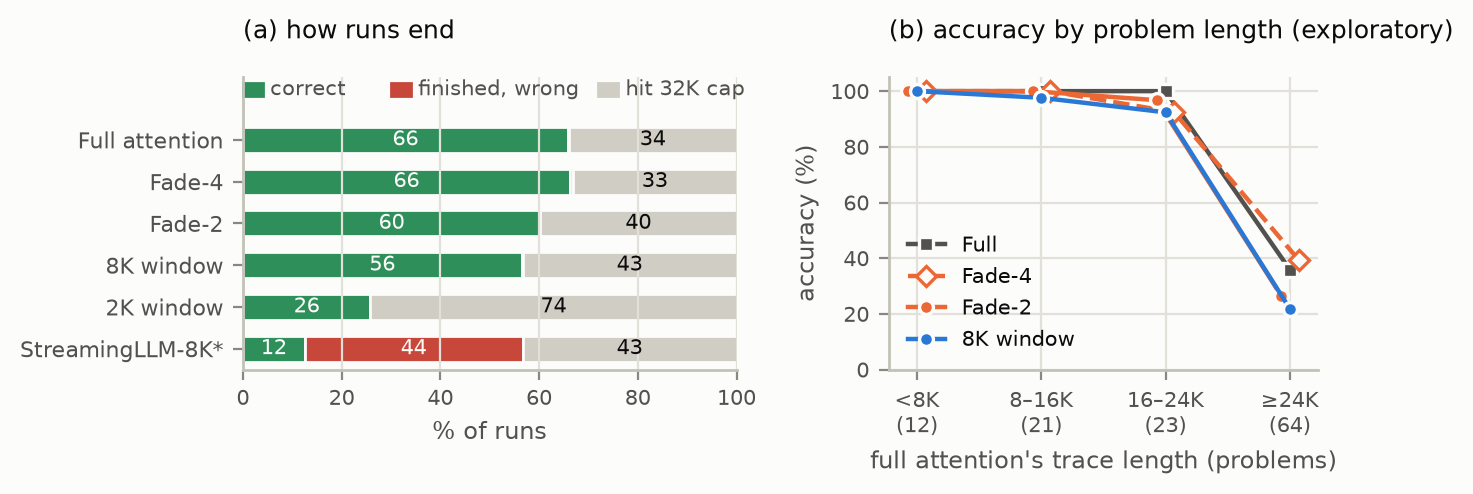
\includegraphics[width=\linewidth]{figures/fig_fade_outcomes.png}
\vspace{-1.4em}
\caption{How runs fail. (a) Share of runs that end correct, finish with a wrong answer, or hit the 32K-token limit (*StreamingLLM-8K: 2 samples per problem). Fade and the windows almost never finish wrong; they fail by running out of tokens. (b) Exploratory: accuracy within bins of full attention's average trace length per problem. All methods are near 100\% on short problems; the loss to full attention appears on problems whose traces exceed 16K tokens.}
\label{fig:outcomes}
\vspace{-0.6em}
\end{figure}

\takeaway{4. How Fade fails: longer reasoning, not wrong answers.} Every finished 2-bit run is correct (289 of 289). The loss comes from runs that hit the token limit (39.8\% vs 34.0\% for full attention), and finished 2-bit runs are about 860 tokens longer. This matches the lengthening reported for aggressive KV compression on dense models~\cite{thinkv,breadthkv}. As Figure~\ref{fig:outcomes}b shows (exploratory), all methods solve the short problems; the loss to full attention appears on problems whose traces exceed 16K tokens, and the gain over the window is clearest beyond 24K, where the window has dropped most of the trace. An exploratory teacher-forced analysis (to 24.6K tokens) is consistent with this: the window's error grows with position while 2-bit Fade's stays nearly flat (Appendix~\ref{app:kl}).

\takeaway{5. The memory savings are real.} A benchmark that stores real packed 2- and 4-bit codes on an A100 matched the analytic memory to within the pre-registered 10\% for every method and context length; at 32K tokens, 2-bit Fade uses 0.83$\times$ the state memory (batch 32) of the 8K window and 0.24$\times$ that of full attention. On peak memory during decoding the ratio is 0.90$\times$ (the prototype's peak is above its state memory, more so for Fade). Our prototype dequantizes in plain PyTorch and is slower than full attention, so we make no speed claim; that needs a fused kernel (Appendix~\ref{app:mem}).

\vspace{-0.6em}
\section{Discussion}
\vspace{-0.4em}
In a hybrid reasoning model, the growing attention memory can be blurred but not cut. Dropping old tokens by position fails, while storing them coarsely works: 4 bits shows no detectable loss, and 2 bits beats a window of matched analytic memory, though a post hoc split puts the whole gain on one of two seed pairs. This is consistent with the exploratory attention maps (not audited), where every head reads far back. Dropping the prompt is far worse still. Fade's failure mode is a weaker version of forgetting's: the model does not answer wrongly; it runs longer and hits the limit more often. Exploratory tests suggest that the hybrid tolerates 2-bit attention memory better than a dense model in total, consistent with it having fewer attention layers to quantize (per quantized layer it is not more tolerant, and we find no evidence that the recurrent layers absorb the noise), and that a short burst of blurring leaves no persistent error detectable above twice the numerical floor (teacher-forced; Appendices~\ref{app:dense}--\ref{app:pulse}).

\paragraph{Limitations.}
\begin{itemize}\setlength{\itemsep}{1pt}\setlength{\topsep}{0pt}
\item \emph{Emulation, no speed claim:} accuracy comes from emulated low-bit storage; memory is analytic, checked against the state memory of a real packed benchmark; peak memory is higher, more so for Fade; there is no fused kernel, and our prototype is slower than full attention.
\item \emph{Scope:} one model, math only, 4 samples per problem (2 for StreamingLLM), one quantizer family and one recent-window size.
\item \emph{Baselines:} our eviction baselines choose tokens by position; score-based eviction such as R-KV~\cite{rkv} and other quantizers such as KVQuant~\cite{kvquant} were not tested.
\item \emph{Fragile primary result:} the 2-bit gain over the window sits entirely in one of two seed pairs (post hoc).
\item \emph{Novelty:} the quantizer and the quantize-versus-evict question are known on dense models~\cite{kivi,breadthkv}; what is new is the hybrid setting and the evidence that its attention needs old tokens in every head.
\end{itemize}

\paragraph{Future work.} \emph{Systems:} a fused low-bit attention kernel in a serving engine (vLLM or SGLang) to measure throughput. \emph{More baselines:} we will compare Fade at matched memory with more baselines: score-based eviction (R-KV~\cite{rkv}, RaaS~\cite{raas}), other quantizers (KVQuant~\cite{kvquant}, SKVQ~\cite{skvq}), methods that mix quantization and eviction (PM-KVQ~\cite{pmkvq}, ThinKV~\cite{thinkv}), and head-aware methods (DuoAttention~\cite{duoattention}). \emph{Policy:} bits that fade gradually with age (8 $\to$ 4 $\to$ 2 $\to$ 1). \emph{Training:} quantization-aware fine-tuning or self-distillation of the 8 FA layers to close the 2-bit gap or reach 1 bit. \emph{Scope:} more hybrid models and more tasks.

\small
\begin{thebibliography}{99}
\setlength{\itemsep}{1pt}

\bibitem{qwen35} Qwen Team. Qwen3.5 model family. \url{https://huggingface.co/Qwen}, 2026.

\bibitem{gdn} Songlin Yang, Jan Kautz, and Ali Hatamizadeh. Gated delta networks: Improving Mamba2 with delta rule. In \emph{ICLR}, 2025. arXiv:2412.06464.

\bibitem{streamingllm} Guangxuan Xiao, Yuandong Tian, Beidi Chen, Song Han, and Mike Lewis. Efficient streaming language models with attention sinks. In \emph{ICLR}, 2024.

\bibitem{kivi} Zirui Liu, Jiayi Yuan, Hongye Jin, Shaochen Zhong, Zhaozhuo Xu, Vladimir Braverman, Beidi Chen, and Xia Hu. KIVI: A tuning-free asymmetric 2bit quantization for KV cache. In \emph{ICML}, 2024. arXiv:2402.02750.

\bibitem{kvquant} Coleman Hooper, Sehoon Kim, Hiva Mohammadzadeh, Michael W. Mahoney, Yakun Sophia Shao, Kurt Keutzer, and Amir Gholami. KVQuant: Towards 10 million context length LLM inference with KV cache quantization. In \emph{NeurIPS}, 2024. arXiv:2401.18079.

\bibitem{skvq} Haojie Duanmu, Zhihang Yuan, Xiuhong Li, Jiangfei Duan, Xingcheng Zhang, and Dahua Lin. SKVQ: Sliding-window key and value cache quantization for large language models. arXiv:2405.06219, 2024.

\bibitem{quarot} Saleh Ashkboos et al. QuaRot: Outlier-free 4-bit inference in rotated LLMs. In \emph{NeurIPS}, 2024. arXiv:2404.00456.

\bibitem{qjl} Amir Zandieh, Majid Daliri, and Insu Han. QJL: 1-bit quantized JL transform for KV cache quantization with zero overhead. arXiv:2406.03482, 2024.

\bibitem{turboquant} Amir Zandieh et al. TurboQuant: Online vector quantization with near-optimal distortion rate. arXiv:2504.19874, 2025.

\bibitem{rkv} Zefan Cai, Wen Xiao, Hanshi Sun, Cheng Luo, et al. R-KV: Redundancy-aware KV cache compression for reasoning models. arXiv:2505.24133, 2025.

\bibitem{raas} Junhao Hu, Wenrui Huang, Weidong Wang, Zhenwen Li, et al. RaaS: Reasoning-aware attention sparsity for efficient LLM reasoning. arXiv:2502.11147, 2025.

\bibitem{pmkvq} Tengxuan Liu, Shiyao Li, Jiayi Yang, Tianchen Zhao, et al. PM-KVQ: Progressive mixed-precision KV cache quantization for long-CoT LLMs. In \emph{ICLR}, 2026. arXiv:2505.18610.

\bibitem{thinkv} Akshat Ramachandran, Marina Neseem, Charbel Sakr, Rangharajan Venkatesan, Brucek Khailany, and Tushar Krishna. ThinKV: Thought-adaptive KV cache compression for efficient reasoning models. arXiv:2510.01290, 2025.

\bibitem{breadthkv} Runguo Li. Spend bytes on breadth: Precision-count trade-offs for decode-time KV compression in long chain-of-thought reasoning. arXiv:2610.05685, 2026.

\bibitem{retrievalheads} Wenhao Wu, Yizhong Wang, Guangxuan Xiao, Hao Peng, and Yao Fu. Retrieval head mechanistically explains long-context factuality. arXiv:2404.15574, 2024.

\bibitem{duoattention} Guangxuan Xiao et al. DuoAttention: Efficient long-context LLM inference with retrieval and streaming heads. In \emph{ICLR}, 2025. arXiv:2410.10819.

\bibitem{razorattention} Hanlin Tang et al. RazorAttention: Efficient KV cache compression through retrieval heads. In \emph{ICLR}, 2025. arXiv:2407.15891.

\bibitem{delethink} Milad Aghajohari, Kamran Chitsaz, Amirhossein Kazemnejad, Sarath Chandar, Alessandro Sordoni, Aaron Courville, and Siva Reddy. The Markovian thinker: Architecture-agnostic linear scaling of reasoning. In \emph{ICLR}, 2026. arXiv:2510.06557.

\bibitem{thinkreset} Fei Ding, Yongkang Zhang, Runhao Liu, Yuhao Liao, et al. ThinkReset: Learnable intermediate interface construction for bounded-context long-horizon reasoning. arXiv:2607.28642, 2026.

\bibitem{kimilinear} Kimi Team. Kimi Linear: An expressive, efficient attention architecture. arXiv:2510.26692, 2025.

\bibitem{qwen3} An Yang et al. Qwen3 technical report. arXiv:2505.09388, 2025.

\bibitem{matharena} Mislav Balunovi\'c et al. MathArena: Evaluating LLMs on uncontaminated math competitions. arXiv:2505.23281, 2025.

\bibitem{hendrycksmath} Dan Hendrycks, Collin Burns, Saurav Kadavath, Akul Arora, Steven Basart, Eric Tang, Dawn Song, and Jacob Steinhardt. Measuring mathematical problem solving with the MATH dataset. In \emph{NeurIPS Datasets and Benchmarks}, 2021.

\bibitem{math500} Hunter Lightman et al. Let's verify step by step. arXiv:2305.20050, 2023.

\end{thebibliography}

\normalsize

\appendix

\section{Motivation: Think-Local and the attention maps}
\label{app:tl}
Think-Local (pre-registered; same 120 problems, sampler and cap; $k{=}4$) restricted each FA layer to the prompt plus the last $W$ generated tokens. Accuracy against full attention (65.8\%): W1K 14.8\% ($-51.0$\pp, $-58.3$ to $-43.8$), W2K 25.8\% ($-40.0$, $-47.1$ to $-32.9$; the registered primary), W4K 42.9\% ($-22.9$, $-28.5$ to $-17.5$), W8K 56.5\% ($-9.4$; added post hoc). Evicting the prompt as well (StreamingLLM-2K) gave 1.2\%. Windowed runs that finished were right (672 of 673 on math); the loss was runs that never finished, and it grew with the length of the derivation.

Exploratory maps on 40 held-out MATH-500 level-5 traces (teacher-forced, not in the test set, not audited): every one of the 32 FA KV heads puts 0.19--0.46 of its attention weight on generated tokens more than 2K back, so no head is local and none is a dedicated far-reader. Keeping 4 heads at full attention and windowing the other 28 leaves 86--94\% of the window's KL, for the 4 most sensitive heads and for each of 5 random sets of 4 (not every set was tested). Keeping the two most sensitive layers (model layers 11 and 15) at full attention still leaves 53\% of it.

\section{Teacher-forced KL sweep}
\label{app:kl}
\begin{figure}[H]
\centering
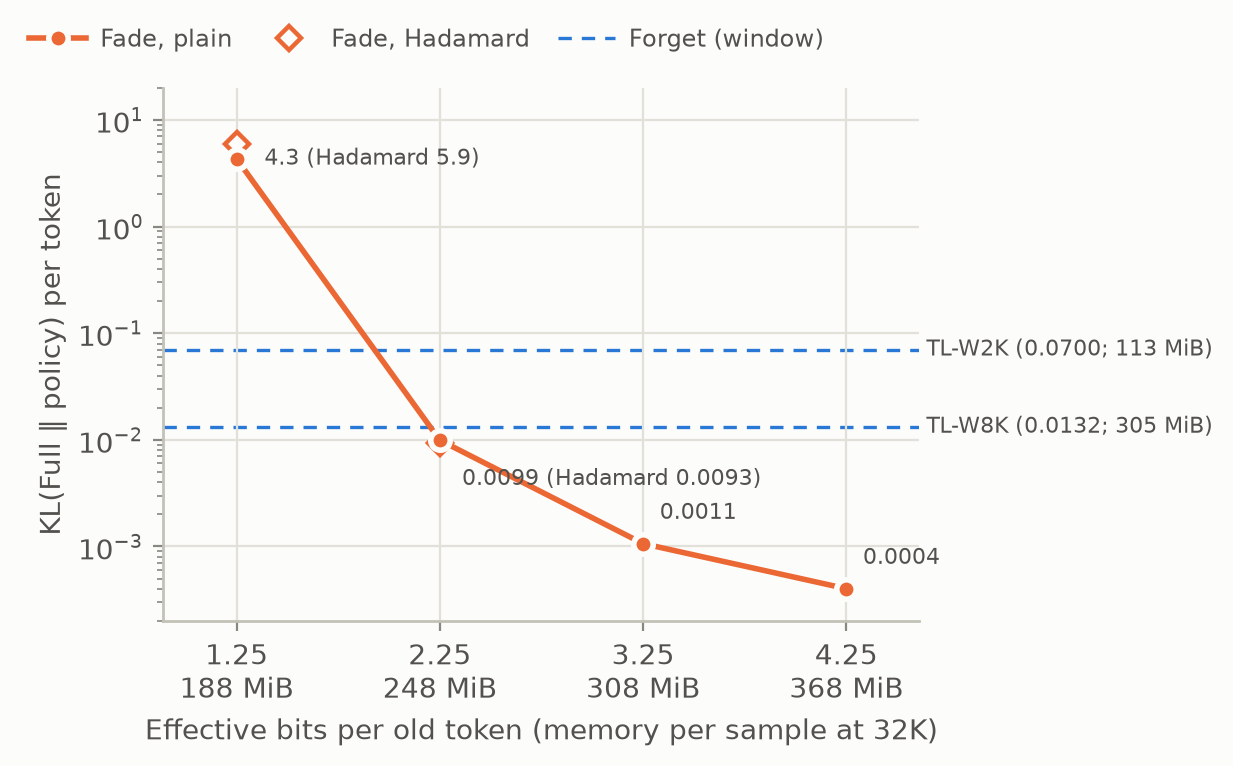
\includegraphics[width=0.55\linewidth]{figures/fig_fade_kl.png}
\vspace{-0.6em}
\caption{Exploratory: teacher-forced KL vs bits per old token on 40 held-out traces, scored from generated token 2,048 up to 24,576; analytic memory at 32K. 2 bits sits just below the 8K window; 1 bit breaks the model.}
\label{fig:kl}
\end{figure}

\paragraph{Teacher-forced view.} On the 40 held-out traces, 2-bit storage keeps the next-token distribution closer to full attention than an 8K window does (KL per token 0.0099 plain and 0.0093 Hadamard vs 0.0132), with less memory, while 4 bits is near-lossless (0.0004) and 1 bit breaks the model (KL $>4$, top-1 agreement 0.12--0.25). The advantage depends on position: below 8K the window is exact and 2 bits is worse; at 8--16K there is no detectable difference; from 8--16K to 16--24.6K the window's KL grows (0.0115 $\to$ 0.0274) while 2-bit plain stays nearly flat (0.0110 $\to$ 0.0121). This is consistent with the decode, where the gain over the window sits in the longest problems, though the decode runs to 32K and the sweep measured nothing beyond 24,576 tokens.
\begin{table}[H]
\caption{KL(full $\|$ policy) per token on 40 held-out traces (841,368 scored tokens, generated positions 2,048 to $\le$24,576), with a trace-level bootstrap CI. Memory: analytic per sample at 32K generated tokens, prompt KV left out. Exploratory; audited.}
\centering
\small
\setlength{\tabcolsep}{3pt}
\begin{tabular}{@{}lccrc@{}}
\toprule
Older tokens & Effective bits & MiB at 32K & KL / token [95\% CI] & Top-1 agreement \\
\midrule
exact (full attention) & 16 & 1,073 & 0 & 1 \\
4-bit plain (Fade-4) & 4.25 & 368 & 0.0004 [0.0004, 0.0004] & 0.995 \\
3-bit plain & 3.25 & 308 & 0.0011 [0.0010, 0.0012] & 0.991 \\
model layers 11, 15 at 4 bits, rest at 2 & 2.75 & 278 & 0.0069 [0.0059, 0.0081] & 0.979 \\
2-bit plain & 2.25 & 248 & 0.0099 [0.0088, 0.0113] & 0.974 \\
2-bit Hadamard (Fade-2) & 2.25 & 248 & 0.0093 [0.0086, 0.0100] & 0.974 \\
2-bit plain, keys before RoPE & 2.25 & 248 & 0.0099 [0.0087, 0.0112] & 0.974 \\
1-bit plain & 1.25 & 188 & 4.32 [4.20, 4.43] & 0.252 \\
1-bit Hadamard & 1.25 & 188 & 5.95 [5.83, 6.06] & 0.124 \\
dropped beyond 8K (TL-W8K) & 0 & 305 & 0.0132 [0.0118, 0.0147] & 0.979 \\
dropped beyond 2K (TL-W2K) & 0 & 113 & 0.0700 [0.0655, 0.0744] & 0.939 \\
\bottomrule
\end{tabular}
\end{table}

Keys or values alone at 2 bits (the other exact) give 0.0033 and 0.0050: both contribute. Quantizing keys before RoPE makes no visible difference at 2 bits (0.0099 vs 0.0099). Hadamard vs plain at 2 bits is a near-tie: paired difference $-0.0007$ [$-0.0014$, $-0.0001$], lower on only 19 of 40 traces. On a second task (40 of Qwen3.5's own Countdown traces), the position pattern repeats (2 bits ties the window at 8--16K and wins at 16--24.6K), but over the whole trace there is no detectable difference from the window, and Hadamard is worse than plain at every position. The layer-mix row is in-sample: layers 11 and 15 were picked from the layer map on the same traces.

\section{Accuracy by problem length}
\label{app:length}
\begin{table}[H]
\caption{Accuracy within bins of full attention's mean trace length per problem (bins from Think-Local; exploratory). Differences in pp, paired by problem, 95\% CI.}
\centering
\small
\setlength{\tabcolsep}{3.5pt}
\begin{tabular}{@{}lrrrrrcc@{}}
\toprule
Full's length & Problems & Full & TL-W8K & Fade-2 & Fade-4 & Fade-2 $-$ TL-W8K & Fade-2 $-$ Full \\
\midrule
$<$8K & 12 & 100 & 100 & 100 & 100 & 0 & 0 \\
8--16K & 21 & 100 & 97.6 & 100 & 100 & $+2.4$ [0, $+6.0$] & 0 \\
16--24K & 23 & 100 & 92.4 & 96.7 & 92.4 & $+4.3$ [$-1.1$, $+9.8$] & $-3.3$ [$-6.5$, $-1.1$] \\
$\ge$24K & 64 & 35.9 & 21.9 & 26.6 & 39.5 & $+4.7$ [$+0.4$, $+9.4$] & $-9.4$ [$-14.5$, $-4.3$] \\
\bottomrule
\end{tabular}
\end{table}

\section{Hybrid vs dense (exploratory)}
\label{app:dense}
Is the hybrid's tolerance special? We teacher-forced dense Qwen3-8B~\cite{qwen3} (36 attention layers, 8 KV heads of dimension 128, 144\,KiB per token) on the same texts, re-tokenized, with the same quantizer. KL is per 1,000 characters, since the tokenizers differ; $r$ is Qwen3.5's KL over Qwen3-8B's, paired over texts. The reading rule was fixed before any Qwen3-8B number.

\begin{table}[H]
\caption{$r$ = KL(Qwen3.5-9B) / KL(Qwen3-8B) per character, 95\% CI; 40 math and 40 Countdown texts written by Qwen3.5.}
\centering
\small
\begin{tabular}{@{}lcc@{}}
\toprule
Config (Qwen3.5's 8 FA layers vs Qwen3-8B) & Math $r$ & Countdown $r$ \\
\midrule
4-bit vs 4-bit, all 36 layers & 0.57 [0.56, 0.58] & 0.58 [0.57, 0.59] \\
2-bit vs 2-bit, all 36 layers & 0.34 [0.32, 0.37] & 0.28 [0.27, 0.29] \\
2-bit vs 2-bit, every 4th dense layer (9 of 36) & 1.34 [1.23, 1.47] & 1.07 [1.02, 1.12] \\
8K window vs 8K window & 0.63 [0.60, 0.66] & 0.61 [0.59, 0.64] \\
2K window vs 2K window & 0.54 [0.52, 0.56] & 0.48 [0.46, 0.49] \\
\bottomrule
\end{tabular}
\end{table}

Against all 36 dense layers at 2 bits, the hybrid drifts about a third as much; against 9 dense layers in the hybrid's 1-in-4 layout, it drifts more (both CIs above 1). The pre-specified reading is ``explained by how many layers are quantized'': the hybrid's lower total drift is consistent with it having fewer attention layers, and per quantized layer it is not more tolerant. The models also differ in training, KV shape and tokenizer, so one pair does not establish the cause. The control quantizes 9 dense layers rather than 8, at one fixed phase; the dense model scores slightly fewer characters per text (0.22\% on math, 0.36\% on Countdown overall); and all texts are teacher-forced and at most 24,576 tokens long. The text is off-policy for the dense model: under full attention it costs Qwen3-8B 0.91 nats per token on math and 0.84 on Countdown (0.36 and 0.44 per character), against 0.36 and 0.35 for Qwen3.5 (0.14 and 0.19 per character), i.e.\ 2.5$\times$ and 2.3$\times$ per character.

One result is unexplained. On the dense model, 2-bit Hadamard gives KL 1.31 per token on math (plain 2-bit: 0.030), growing with distance, while on the hybrid the two variants are close. Exploratory diagnostics on the first 4 dense math traces (added after the dense rows were seen; no CI) show where it appears: only when keys are Hadamard-rotated at 2 bits (keys alone 1.11; values alone 0.0013, below plain 2-bit values at 0.0032; 4-bit Hadamard 0.0007, about the same as 4-bit plain at 0.0007, though slightly higher on each of the 4 traces). The cause is not established. Fade-2 uses the Hadamard variant only on the hybrid, where it is a near-tie with plain.

\section{Where a blurred memory's error lives (exploratory)}
\label{app:pulse}
On 10 long traces (of only 2 problems, selected by a registered rule), queries at generated positions 8,192--9,215 read old tokens at 2 bits, and every other query reads them exactly. A no-op run through the same code gives the bf16 noise floor. At the pulse's end, we either restore the exact recurrent state (so only the attention K/V written during the pulse carry error) or restore the exact K/V (so only the recurrent state does). From 1,024 tokens after the pulse, KL is 1.30$\times$ the floor with both carriers, 1.20$\times$ with the cache alone and 1.10$\times$ with the recurrent state alone, so neither keeps the error above the pre-specified 2$\times$ floor: ``no persistent error detectable above numerical noise''. This means below 2$\times$ the floor, not absent: all runs stay slightly above it in every trace. The rule compares single-carrier branches with a floor whose noise flows through both carriers, so it leans toward the null; with 2 problems there is no CI; and one smoke on a registered trace (aime25\_10 \#0, shortened spans) was seen before the floor rule was fixed. The dense model's error also fades but stays at 1.82$\times$ its floor with all 36 layers quantized. The test is teacher-forced; in free-running decoding, one changed token changes all the text that follows.

\section{All comparisons and details of the main results}
\label{app:details}
In the appendices, TL-W$W$ (Think-Local window) denotes the window of the last $W$ generated tokens plus the prompt. Registered contrasts are read with the pre-registered wording rules; Q1 has a 5\pp\ non-inferiority margin.

\begin{table}[H]
\caption{All paired contrasts (accuracy difference in percentage points, paired by problem). Memory ratio: analytic mean memory per sample, first cell over second. StreamingLLM-8K rows use samples 0--1 of both cells; their memory ratios leave out the prompt's KV, which the other cells keep and StreamingLLM evicts, so on true memory they are slightly higher (median prompt 3.6\,MiB).}
\label{tab:allcontrasts}
\centering
\small
\setlength{\tabcolsep}{4pt}
\begin{tabularx}{\linewidth}{@{}llcY@{}}
\toprule
Contrast & Difference [95\% CI] & Memory & Reading \\
\midrule
Fade-4 $-$ Full (Q2) & $+0.4$ \ci{-2.7}{+3.5} & 0.37$\times$ & no detectable difference \\
Fade-2 $-$ Full (Q1) & $-5.6$ \ci{-8.8}{-2.7} & 0.27$\times$ & worse; not shown non-inferior (5\pp\ margin) \\
\textbf{Fade-2 $-$ TL-W8K (primary)} & $+3.8$ \ci{+1.0}{+6.7} & 0.70$\times$ & better than an 8K window at matched memory \\
\quad seeds 0--1 only (post hoc) & $+7.9$ \ci{+4.2}{+11.7} & & \multirow{2}{=}{the whole gain sits in one seed pair} \\
\quad seeds 2--3 only (post hoc) & $-0.4$ \ci{-4.6}{+3.3} & & \\
Fade-2 $-$ StreamingLLM-8K (SL1) & $+49.2$ \ci{+41.2}{+57.1} & 0.71$\times$ & better than StreamingLLM-8K at matched memory \\
Fade-4 $-$ StreamingLLM-8K (SL2) & $+54.6$ \ci{+47.1}{+62.5} & 0.97$\times$ & better than StreamingLLM-8K at matched memory \\
TL-W8K $-$ StreamingLLM-8K (descr.) & $+41.2$ \ci{+33.8}{+48.8} & 1.01$\times$ & the two differ by design only in keeping the prompt \\
Fade-4 $-$ TL-W2K (Q2) & $+40.4$ \ci{+33.3}{+47.5} & 2.5$\times$ & better; TL-W2K is 40\pp\ below Full \\
Fade-4 $-$ TL-W8K (post hoc) & $+9.8$ \ci{+5.6}{+14.2} & 0.96$\times$ & better than the window at slightly less memory \\
\bottomrule
\end{tabularx}
\end{table}

\paragraph{Against full attention.} 4-bit Fade: no detectable change in finished rate ($+0.8$\pp, $-2.1$ to $+3.8$; cap hits 33.1\% vs 34.0\%) and no detectable change in the length of finished runs ($-231$ tokens, $-678$ to $+204$). 2-bit Fade: the CI's lower end ($-8.8$\pp) is beyond the 5\pp\ margin, so non-inferiority is not shown. Across bits (the Q2 curve; descriptive), accuracy goes 25.8\% (0 bits, TL-W2K) $\to$ 60.2\% (2.25) $\to$ 66.2\% (4.25) $\to$ 65.8\% (16, full).

\paragraph{Against an 8K window (primary).} At the 32K cap the memory ratio is 0.81$\times$ (248 vs 305\,MiB). 2-bit Fade also finishes more often ($+3.5$\pp, $+0.8$ to $+6.3$). The post hoc split by seed pair was suggested by the auditor; two seed pairs cannot separate seed-pair noise from a seed-linked effect, so we report the registered pooled verdict with this caveat. In the exploratory split by problem length (Appendix~\ref{app:length}; no multiplicity control), the gain sits in problems whose full-attention traces exceed 24K tokens ($+4.7$\pp, $+0.4$ to $+9.4$), the only bin where the CI excludes zero.

\paragraph{How 2 bits fails.} The finished rate drops by 5.8\pp\ against full attention ($-9.0$ to $-2.9$), and finished 2-bit runs are 857 tokens longer ($+320$ to $+1{,}406$, over the 88 problems where both cells finish at least once). In the length bins, the loss to full attention is largest beyond 24K ($-9.4$\pp).

\paragraph{Against StreamingLLM-8K.} StreamingLLM-8K ran 2 samples per problem (seeds 0--1); its analysis (\texttt{fade\_sl.py}) was registered before any of its runs, and a StreamingLLM-4K cell (contrasts SL5 and SL6) was registered but not run. Its 12.5\% (7.5 to 17.9) is in the range we expected before the run (roughly 10--20\%). On the same two samples, Full, Fade-4, Fade-2 and TL-W8K score 65.4, 67.1, 61.7 and 53.8\%. Using all four Fade samples gives the same verdict (SL1 $+47.7$\pp, $+40.0$ to $+55.2$; sensitivity analysis). Descriptively, full attention is $+52.9$\pp\ ($+45.0$ to $+60.8$) above StreamingLLM-8K. SL1 and SL2 compare runs from one build of the decode loop; the descriptive contrasts, like the primary, cross builds. StreamingLLM-8K hits the cap about as often as TL-W8K on these samples (43.3\% vs 45.8\%; finished-rate difference $-2.5$\pp, $-8.3$ to $+2.9$), but most of its finished runs are wrong (106 of 136, against 1 of 130 for TL-W8K). Its 30 correct runs are the 28 runs short enough never to fill the 8,196-token window (these match full attention at the same seed in length and answer, a check on the implementation) and 2 of the 212 runs that did fill it. In Think-Local, the same eviction at a 2K window gave 1.2\% accuracy against TL-W2K's 25.8\% ($+24.6$\pp\ for keeping the prompt, $+18.3$ to $+31.3$). Analytic memory leaves the prompt out for every cell; counting the prompt's KV (still analytic), cells that keep the prompt (all but StreamingLLM) hold a median of about 3.6\,MiB more per sample (median prompt ${\approx}$116 tokens; largest 25.7\,MiB).

\section{Measured memory}
\label{app:mem}
To check the analytic accounting, a benchmark (\texttt{fade\_mem.py}, registered before any of its numbers) stores real packed 2- and 4-bit codes with their scales on an A100 and dequantizes them before attention. A correctness gate ran first: the packed values equal the emulated ones exactly, and over 2,752 teacher-forced steps packed decoding stays within the registered gate of 2$\times$ the bf16 kernel noise floor of the emulated policy (mean KL 1.03$\times$ the floor for Fade-4 and 1.18$\times$ for Fade-2; for Fade-2 the largest logit difference, 16.4, exceeds the floor's 9.2). The benchmark then built each cell's decode state at a total context of 8K, 16K and 32K tokens and batch 1, 8 and 32 (45 configurations, none out of memory) and ran 128 decode steps. The pre-registered check passed: at batch 1 and 32, measured state memory per sample, after removing the capacity the benchmark allocates beyond what the policy holds, is within 10\% of the analytic count for every cell (Eq.~\ref{eq:mem} plus the prompt's KV; for StreamingLLM-8K, which holds no separate prompt, its ring of at most 8,196 slots plus the GDN state; largest deviation $+7.5$\%, 2-bit Fade at 8K and batch 1; at batch 32, all within 0.8\%). At 32K and batch 32, resident state memory per sample, including a 128-token prompt, is 1,082\,MiB for full attention, 378 for Fade-4, 258 for Fade-2, 311 for TL-W8K and 307 for StreamingLLM-8K; peak memory per sample during decoding, above the weights, is 1,085, 402, 282, 314 and 310\,MiB. On state memory, the ratios Fade-2/TL-W8K 0.83, Fade-2/StreamingLLM-8K 0.84, Fade-2/Full 0.24 and Fade-4/Full 0.35 are within 0.02 of the analytic ones at the same context (0.81, 0.82, 0.23, 0.35); on peak memory they are 0.90, 0.91, 0.26 and 0.37. Speed is not claimed: this prototype dequantizes in unfused PyTorch and is slower than full attention, from 1.5$\times$ (8K, batch 1) to 18$\times$ per step (32K, batch 32: 998\,ms for Fade-2 and 561 for Fade-4 vs 55 for full attention); these are upper bounds, and any speed claim needs a fused kernel. The benchmark only builds the state and runs 128 decode steps per configuration.

\section{Implementation, checks and statistics}
\label{app:impl}
\paragraph{Model and quantizer.} Each of Qwen3.5-9B's 8 FA layers has 4 KV heads of dimension 256, so a token costs $2\times4\times256\times2$\,B $= 4$\,KiB per layer and 32\,KiB over the 8 layers. Keys are cached after RoPE, which rotates 64 of the 256 dimensions. Fade quantizes a block of $G{=}128$ generated tokens once, irreversibly, when its last token is $R{=}2{,}048$ tokens old, so the most recent 2,048--2,175 generated tokens are always exact. Keys are quantized per channel over each 128-token block and values per token in groups of 128 channels, each group with an fp16 scale $s$ and zero point $z$ ($b{+}0.25$ effective bits). The Hadamard variant rotates each 256-dimensional head vector with a normalized Hadamard matrix, quantizes keys and values per token in groups of 128, and rotates back. Codes $c$ are dequantized as $\hat{k} = s\,c + z$.

\paragraph{Correctness checks.} Before any experiment: $b{=}16$ is bit-identical to full attention; masks and in-place quantization match an fp64 per-query oracle (max error $1.5{\times}10^{-14}$); and in batched decoding each sample's blocks age on their own schedule, bit-exactly.

\paragraph{Configuration choice.} Cell A, the 2-bit variant with the lowest teacher-forced KL, is 2-bit Hadamard (0.0093 vs 0.0099 for plain, a near-tie). Cell B would be a variant below 2 bits whose KL is at most the 8K window's; neither 1-bit variant came close (KL 4.3 and 5.9 vs 0.0132), so Cell B is the pre-registered fallback, 4-bit plain. The sweep used 40 held-out MATH-500 level-5 traces, not in the test set.

\paragraph{Decoding and statistics.} Thinking mode with temperature 1.0, top-$p$ 0.95, top-$k$ 20 and presence penalty 1.5, under a 32,768-token cap; answers are scored automatically. Seeds are shared across cells only nominally (batch composition changes bf16 reduction order), so every contrast is paired by problem. CIs are two-sided 95\% intervals from a cluster bootstrap over problems, stratified by dataset (10,000 resamples). The registered questions: the primary contrast Fade-2 $-$ TL-W8K at matched memory; Q1, Fade-2 $-$ full attention with a 5\pp\ non-inferiority margin; Q2, the curve from 0 to 16 bits; Q3, token counts.

\paragraph{Software and runs.} Hugging Face Transformers 5.19 with PyTorch 2.13 (CUDA 13.0) and the \texttt{fla} 0.6.0 kernels for GDN, in bf16, with a continuous-batching pool. Full, TL and Fade-4/Fade-2 each have 480 runs, and StreamingLLM-8K has 240. The full-attention and window runs are reused from Think-Local; Fade's runs used a later build of the same loop. The new Fade decodes took 11.5 GPU-hours on NVIDIA A100-80GB GPUs, and all of this project's runs about 16 GPU-hours plus 2.7 for StreamingLLM-8K and 0.5 for the memory benchmark, on the lab's own GPUs (no paid compute).

\paragraph{Other limitations.} The cells were picked by teacher-forced KL, and Hadamard vs plain at 2 bits was a near-tie that did not transfer to a second task (Countdown, where Hadamard was worse at every position); plain 2-bit was not decoded. Fade also ran on a later build of the decode loop than the reused baselines.

\section{Pre-registration, audits and compute}
\label{app:prereg}
The Fade analysis plan (\texttt{prereg\_fade.md}) fixed the questions, the cell-selection rule, the primary and secondary contrasts, the verdict wording and the analysis script (\texttt{fade\_stats.py}) before any decode result; changes after that are logged with timestamps and labelled post hoc. The headline numbers are the registered $k{=}4$ rerun; the audited $k{=}2$ interim gave the same verdicts (primary $+5.2$\pp, $+1.5$ to $+9.0$; Q1 $-4.2$\pp, $-7.7$ to $-0.8$). An independent audit agent reproduced every decode, sweep, dense and pulse number from the raw rows and passed each step after fixes to wording and caveats. The StreamingLLM-8K analysis (\texttt{fade\_sl.py}) was registered before any of its runs; the audit agent reproduced its output and every StreamingLLM-8K number and passed it after wording fixes (\texttt{AUDIT\_sl.md}). The memory benchmark's check was registered before any GPU number; its 32K configurations ran alongside the correctness gate rather than after it (the gate passed). The audit agent reproduced its analysis and passed it after wording fixes (\texttt{AUDIT\_mem.md}). Compute on A100-80GB (wall-clock $\times$ GPUs): Fade decodes 11.5 GPU-hours, KL sweep and smokes ${\approx}$0.9, attention maps ${\approx}$1.7, dense comparison ${\approx}$1.2, pulse ${\approx}$0.1 (the later Qwen3.5 NLL and dense diagnostic runs are not counted), StreamingLLM-8K 2.7, memory benchmark 0.5; Think-Local's reused runs took 35.3 GPU-hours. No paid compute was used.

\end{document}
